\section{Einleitung und Lernziele}
Ziel des Labs ist es das Zusammenspiel grundlegender Internetdienste zu
veranschaulichen. Für die erfolgreiche Durchführung der Übung sind folgende
Voraussetzungen von Vorteil:
\begin{itemize}
  \item Grundlagen Linux mit Debian/Ubuntu
  \item Grundlagen TCP/IP, IP-Subnetting und Routing
  \item Grundlagen in Netzwerktopologien und Umgang mit der
  Virtualisierungssoftware VMware
\end{itemize}

In der Übung werden die folgenden Inhalte praktisch vermittelt:
\begin{itemize}
  \item Einrichtung und Konzeption von IP-basierten Netzwerken
  \item Inbetriebnahme eines Servers für Internetdienste unter Linux
  \item Konzepte zur Planung und Einrichtung von privaten und öffentlichen
  LAN-Zugängen mittels Routing und NAT auf Basis von pfSense.
  \item Konzeption und Aufbau von internen DNS-Strukturen und das Verfahren
  zur dezentralen Administration mittels "`Domain Delegation"' mit bind9.
  \item Konzeption und Aufbau einer intranetfähigen Mailserverumgebung auf Basis
  von Postfix
  \item Konzeption und Aufbau einer Intranet Website auf Basis von Apache2
  \item Fehleranalyse im Umgang mit Linux-Systemen in TCP/IP-Netzwerken
  \item {\bf Optional:} Installation und Einrichtung von hochverfügbaren Routern
  mit pf und CARP
  \item {\bf Optional:} Einrichtung eines Monitoringsystems zur Überwachung des
  Laboraufbaus mit OpenNMS
\end{itemize}

Diese Laborumgebung wird mit den Studierenden gemeinsam aufgebaut und
eingerichtet. Für jedes IP-Subnetz konfiguriert jede Lerngruppe eine eigene
DNS-Zone mit einem Intranet Web- und Mailserver. Der Internetzugang soll durch
einen zentralen Router realisiert werden. Der Router hat dabei die Aufgabe NAT
für die privaten Sub-Netze durchzuführen. Zusätzlich sollen DNS-Anfragen ins
Internet über einen zentralen Router realisiert werden. Im Abschluss werden
erweiterte Konfigurationen für Mail-, Web- und DNS-Dienste konfiguriert und
eingerichtet. Um dieses Ziel zu erreichen wird der Laboraufbau in den folgenden
Abschnitten dokumentiert.

\section{Lab Dokumentation}
Der Versuchsaufbau wird im TK-Labor durchgeführt. Jede Lerngruppe
bestehend aus maximal drei Studierenden und erhält ein eigenes privates IPv4
Netz. Es können bis zu 16 Gruppen gebildet werden. Jede Gruppe kann 13
Netzwerkgeräte pro Subnetz einrichten. Die erste Adresse wird für den Router ins
Internet reserviert. Zusätzlich erhält jede Lerngruppe eine Sub-Domain für die
sie verantwortlich ist. Für diese Sub-Domains sind DNS-Server mit entsprechenden
Zonen einzurichten. Die Server sollen in den Zonen per DNS erreichbar sein. Die
IP-Adressen und Domains sind dabei wie folgt eingeteilt:

\begin{tabular}[t]{l l l l l l}
\hline
Netz-ID & Router & Srv1 & Srv2 & Broadcast & Sub-Domain \\
\hline
\textcolor{red}{192.168.1.0} & .1 & .2 & .3 & \textcolor{red}{.15} &
beta.tklabor.site \\ \textcolor{red}{192.168.1.16} & .17 & .18 & .19 &
\textcolor{red}{.31} & antares.tklabor.site \\
\textcolor{red}{192.168.1.32} & .33 & .34 & .35 & \textcolor{red}{.47} &
orion.tklabor.site \\
\textcolor{red}{192.168.1.48} & .49 & .50 & .51 & \textcolor{red}{.63} &
vogsphere.tklabor.site \\
\hline
\textcolor{red}{192.168.1.64} & .65 & .66 & .67 & \textcolor{red}{.79} &
frogstar.tklabor.site \\
\textcolor{red}{192.168.1.80} & .81 & .82 & .83 & \textcolor{red}{.95} &
epun.tklabor.site \\
\textcolor{red}{192.168.1.96} & .97 & .98 & .99 & \textcolor{red}{.111} &
earth.tklabor.site \\
\textcolor{red}{192.168.1.112} & .113 & .114 & .115 & \textcolor{red}{.127} &
earth2.tklabor.site \\
\hline
\textcolor{red}{192.168.1.128} & .129 & .130 & .131 & \textcolor{red}{.143} &
fallia.tklabor.site \\
\textcolor{red}{192.168.1.144} & .145 & .146 & .147 & \textcolor{red}{.159} &
magrathea.tklabor.site \\
\textcolor{red}{192.168.1.160} & .161 & .162 & .163 & \textcolor{red}{.175} &
lamuella.tklabor.site \\
\textcolor{red}{192.168.1.176} & .177 & .178 & .179 & \textcolor{red}{.191} &
kria.tklabor.site \\
\hline
\textcolor{red}{192.168.1.192} & .193 & .194 & .195 & \textcolor{red}{.207} &
zarss.tklabor.site \\
\textcolor{red}{192.168.1.208} & .209 & .210 & .211 & \textcolor{red}{.223} &
rupert.tklabor.site \\
\textcolor{red}{192.168.1.224} & .225 & .226 & .227 & \textcolor{red}{.239} &
eadrax.tklabor.site \\
\textcolor{red}{192.168.1.240} & .241 & .242 & .243 & \textcolor{red}{.255} &
thesun.tklabor.site \\
\hline
\end{tabular}
\newline
\newline
Ein zentraler Router stellt den Internetzugang für das Labornetzwerk zur
verfügung. Die Konfiguration des zentralen Routers soll mit den Studierenden
gemeinsam erarbeitet werden.

\begin{figure}[H]
 	\centering
 		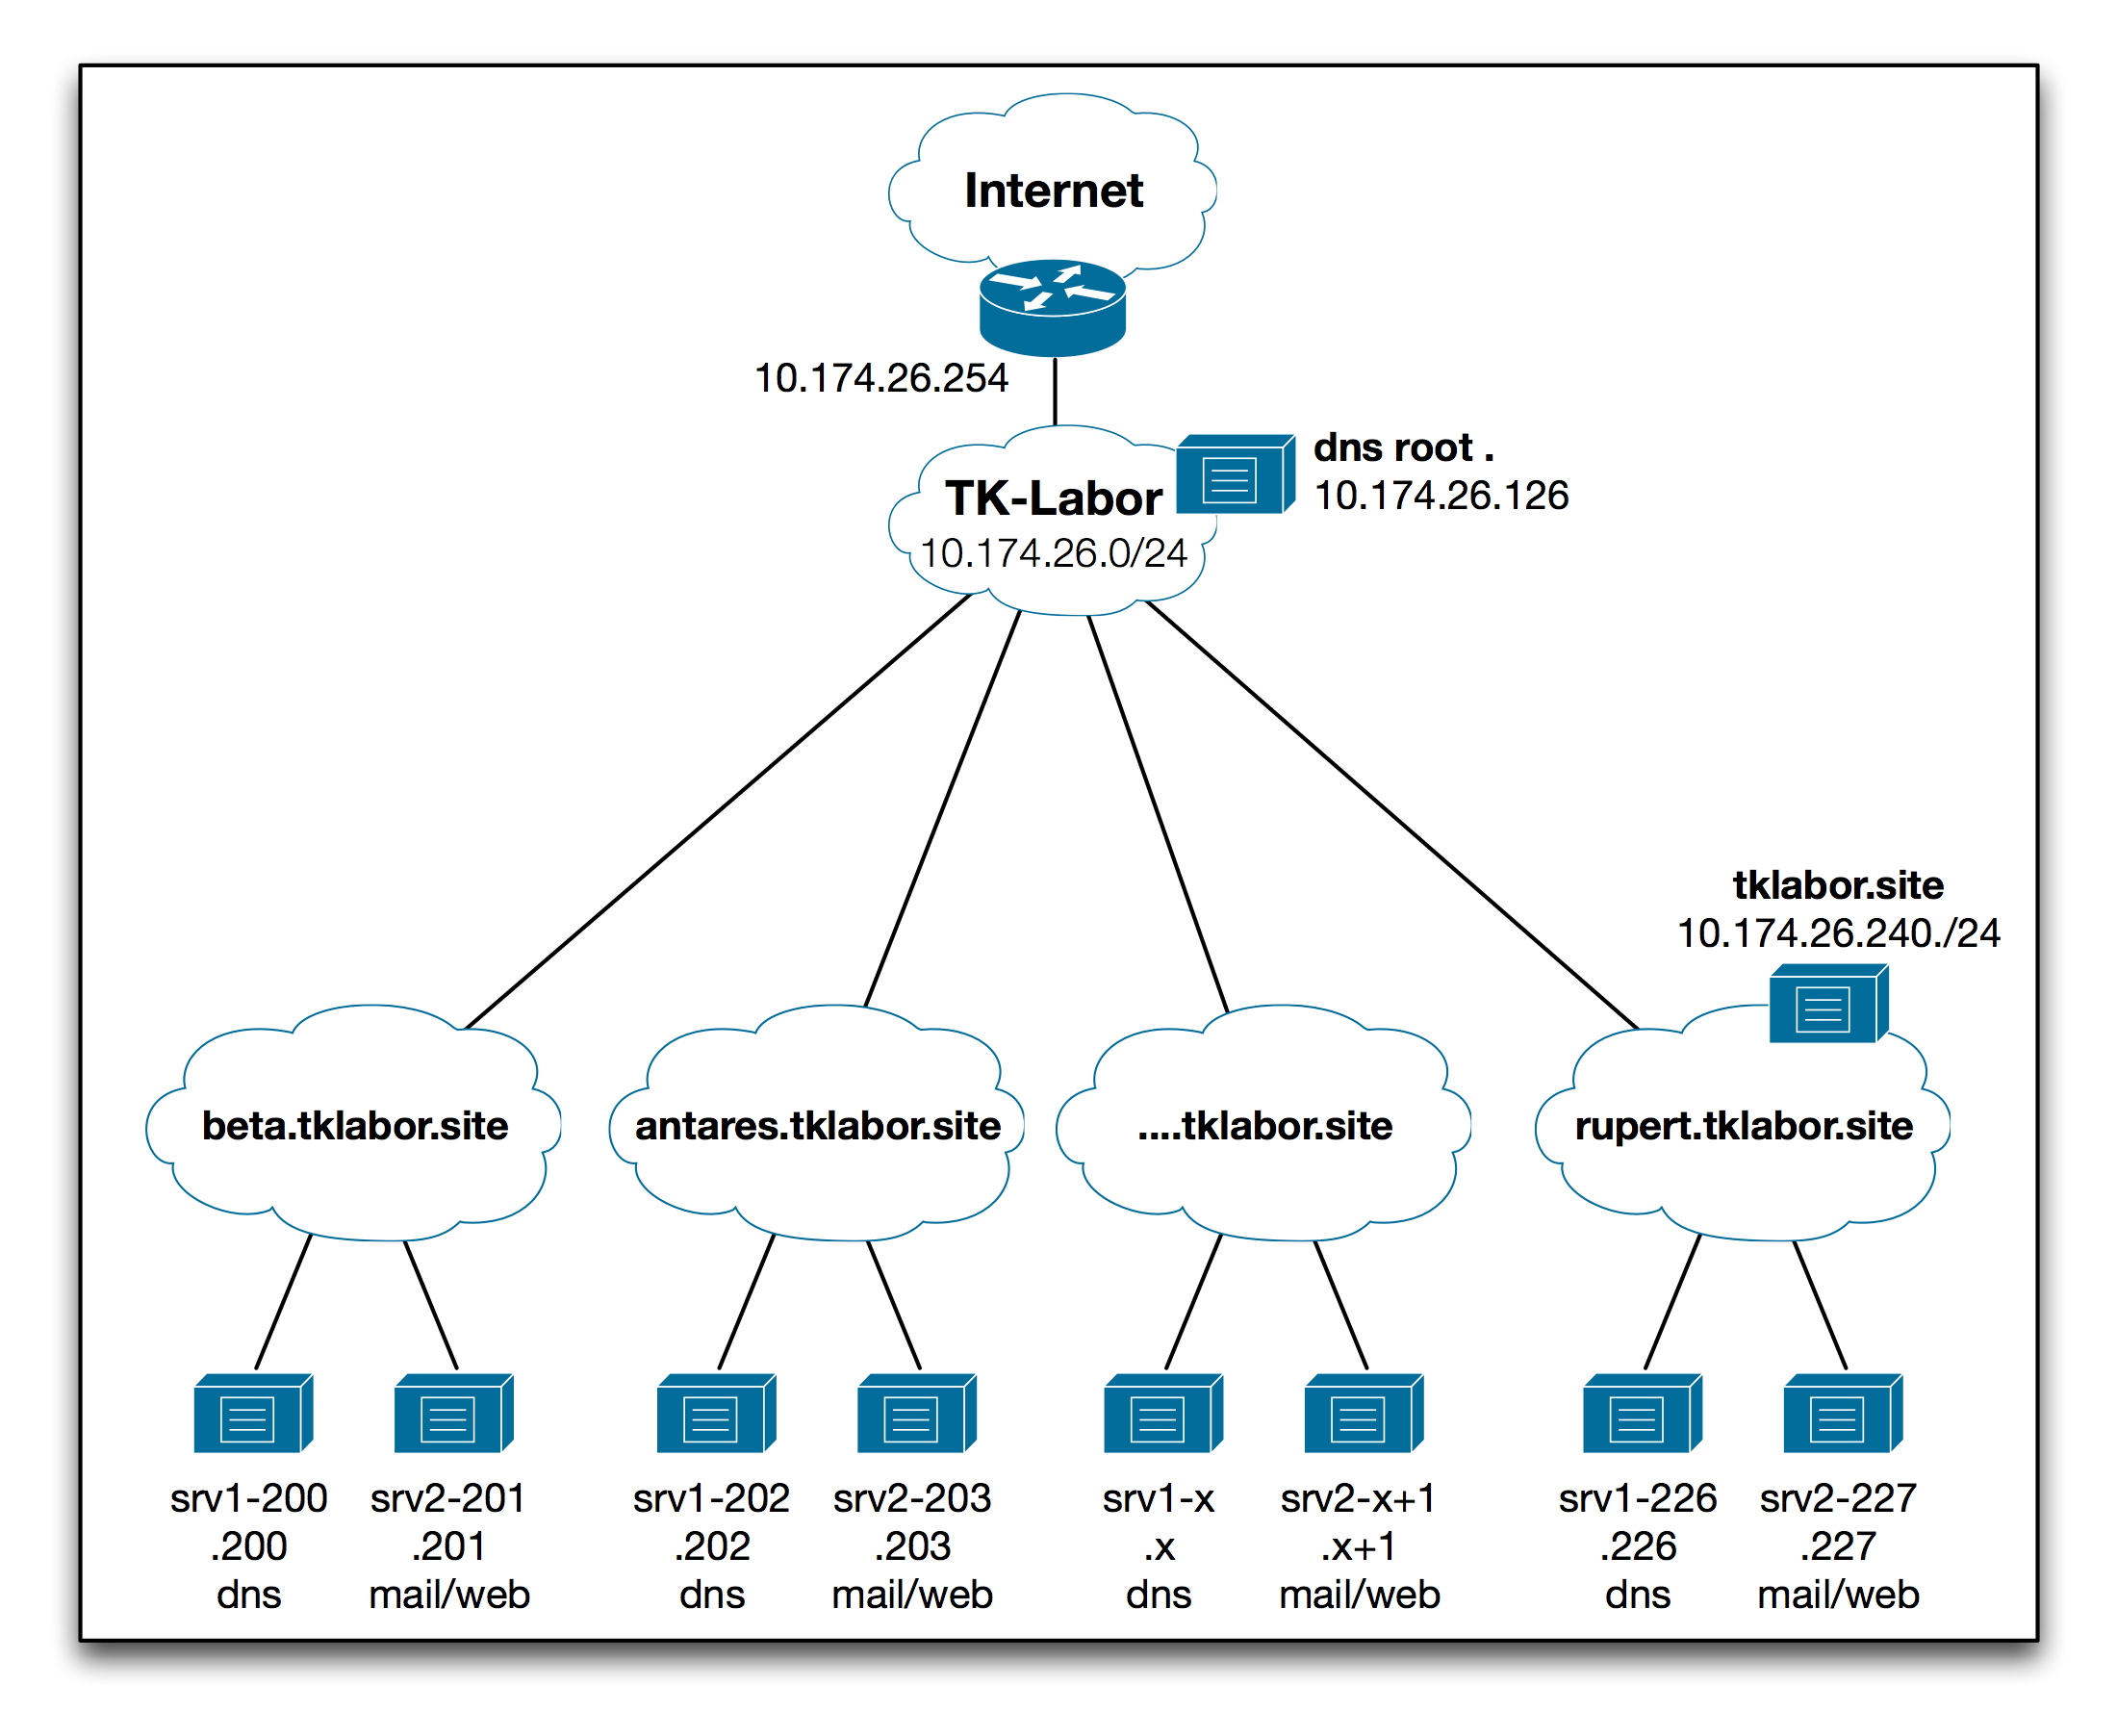
\includegraphics[width=1.0\textwidth]{images/lab-netzplan.png}
 		\caption{Netzplan zum Laboraufbau}
 	\label{fig:chap-labdocu-netzplan}
\end{figure}

Anhand der Abbildung \ref{fig:chap-labdocu-netzplan} sollen die Studierenden
folgende Fragestellung beantworten:

\begin{itemize}
  \item Wie kann eine Kommunikation der Subnetze der Lerngruppen untereinander
  hergestellt werden?
  \item Wie kann ein zentraler Internetzugang realisiert werden? 
  \item Wie muss eine NAT-Konfiguration aussehen und was passiert hiert?
  \item Wie kann die Funktionsfähigkeit der Konfiguration auf Layer-3 überprüft
  werden?
  \item Wie muss die Konfiguration der Server als auch des zentralen Routers
  aussehen, damit DNS-Abfragen über den zentralen Router erfolgen?
  \item Diskutieren Sie Vor- und Nachteile eines zentralen DNS-Zugangs?
  \item Diskutieren Sie Vor- und Nachteile eines Internetzugangs mittels NAT? 
\end{itemize}

Der Versuchsaufbau findet im Raum C106 statt. Die entsprechende
Konfigurationen für die Lerngruppen ist wie folgt vorgesehen:
\begin{figure}[H]
 	\centering
 		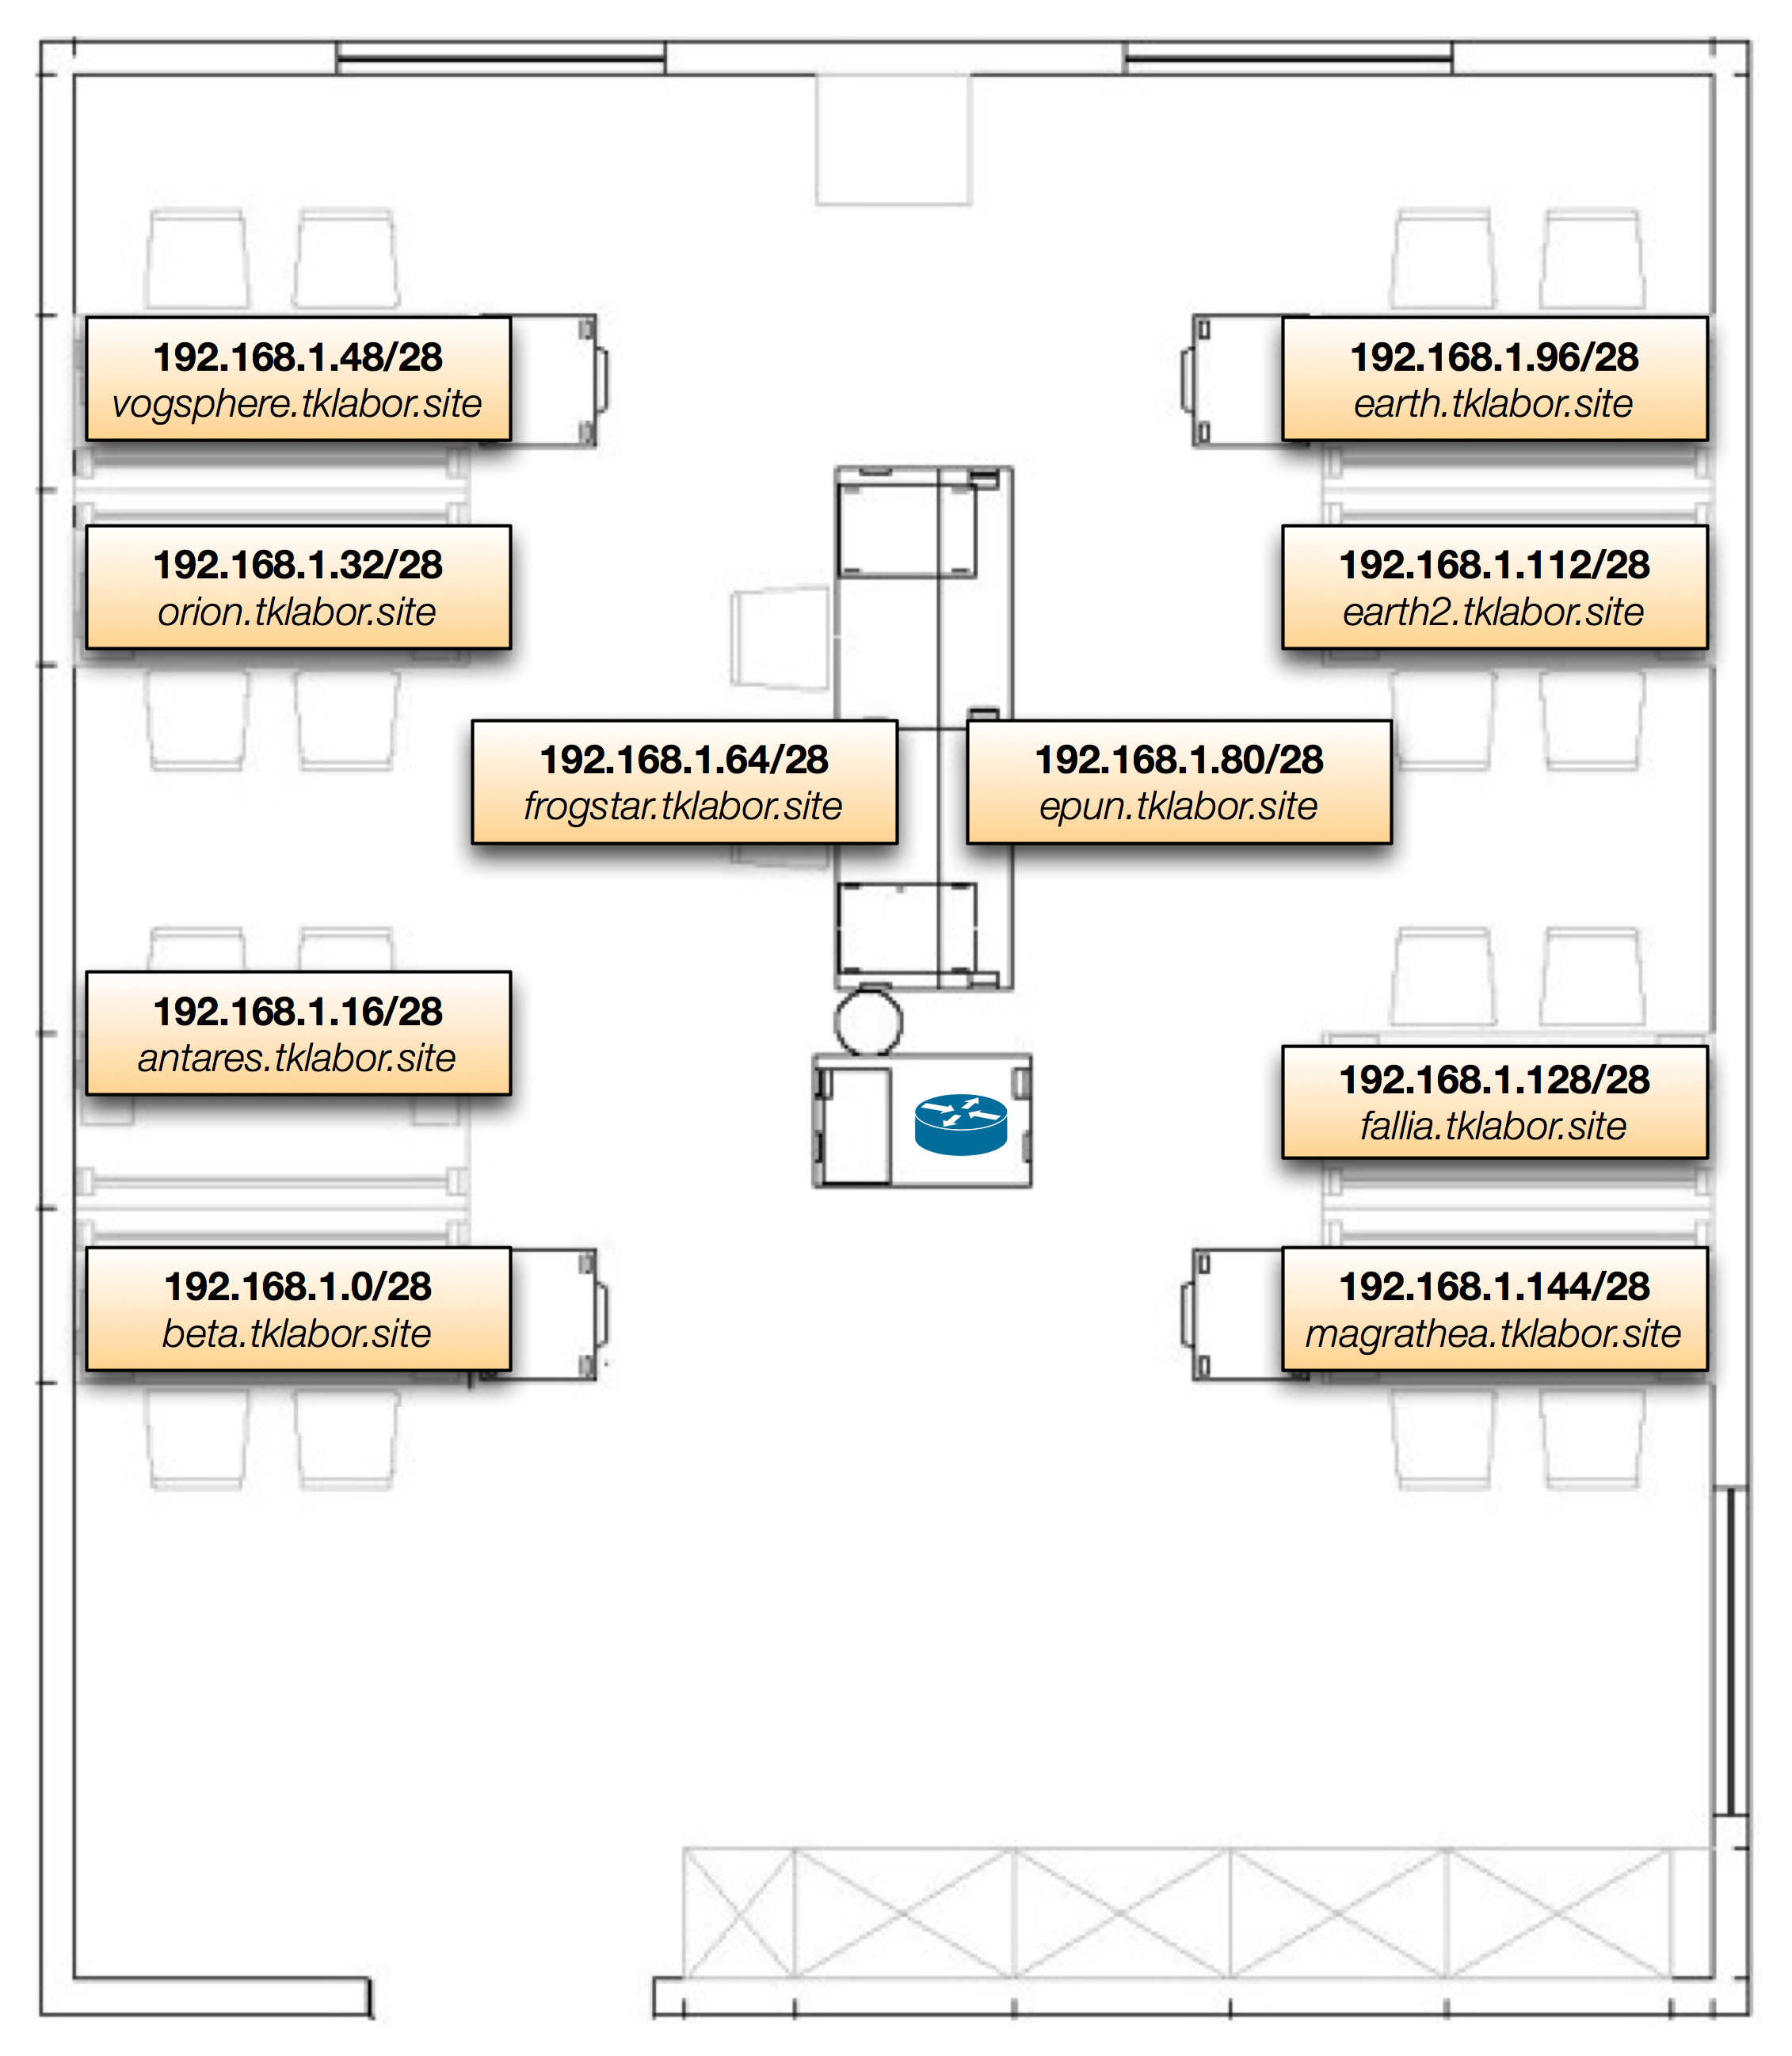
\includegraphics[width=1.0\textwidth]{images/lab-aufbau.png}
 		\caption{Verteilung der Netze und Domains im TK-Labor}
 	\label{fig:chap-labdocu-aufbau}
\end{figure}
